\documentclass[11pt]{article}
\usepackage[margin=0.8in]{geometry}
\usepackage{graphicx}
\usepackage{booktabs}
\usepackage{float}
\usepackage{xurl}

\newcommand{\figsource}[1]{\par\smallskip\noindent{\footnotesize Source program: \texttt{\detokenize{#1}}.}}

\title{Head-Echo RDMF Run v0.2.8}
\author{}
\date{2026-06-13}

\begin{document}
\maketitle

% Auto-generated by fit_ballistic_head_trail_correlated_appendix.py
% trajectory_fit_version: 0.2.8
% trajectory_fit_version_description: Selected head-echo correlated ballistic fit using AoD-steered TX combining, receive-polarization matching, range interpolation by 4, 16x FFT over the interpolated code length, sparse-fit residual voltage, and manual range/Doppler selections from the rinterp4/zp16 RDMF candidate GUI.
\newcommand{\CorrFitNHead}{186}
\newcommand{\CorrFitNHeadRange}{179}
\newcommand{\CorrFitNHeadDoppler}{151}
\newcommand{\CorrFitNTrail}{146}
\newcommand{\CorrFitNResiduals}{768}
\newcommand{\CorrFitReducedChiSq}{3.38}
\newcommand{\CorrFitHeadCoherentCodes}{1}
\newcommand{\CorrFitHeadIncoherentSpectra}{2}
\newcommand{\CorrFitHeadStepCodes}{1}
\newcommand{\CorrFitHeadNeighborCorrelation}{0.50}
\newcommand{\CorrFitHeadNeighborPairs}{296}
\newcommand{\CorrFitTrailCoherentCodes}{8}
\newcommand{\CorrFitTrailCorrelationGateKm}{3.0}
\newcommand{\CorrFitTrailSameGatePairs}{0}
\newcommand{\CorrFitTrailDifferentGateOverlapPairs}{0}
\newcommand{\CorrFitDeltaPositionKm}{4.27}
\newcommand{\CorrFitDeltaVelocityMps}{942.1}
\newcommand{\CorrFitCdAreaMass}{4.021e-04}
\newcommand{\CorrFitBodyDiameterM}{1.6}
\newcommand{\CorrFitBodyMassTon}{5.0}
\newcommand{\CorrFitTrailMedianKm}{1.88}
\newcommand{\CorrFitOldOrbitA}{5.78}
\newcommand{\CorrFitNewOrbitA}{6.07}
\newcommand{\CorrFitOldOrbitE}{0.892}
\newcommand{\CorrFitNewOrbitE}{0.900}
\newcommand{\CorrFitOldOrbitI}{37.39}
\newcommand{\CorrFitNewOrbitI}{36.62}
\newcommand{\CorrFitOldOrbitQ}{0.625}
\newcommand{\CorrFitNewOrbitQ}{0.607}

% trajectory_fit_version: 0.2.8
% trajectory_fit_version_description: Selected head-echo correlated ballistic fit using AoD-steered TX combining, receive-polarization matching, range interpolation by 4, 16x FFT over the interpolated code length, sparse-fit residual voltage, and manual range/Doppler selections from the rinterp4/zp16 RDMF candidate GUI.
% Generated by reports/generate_orbit_source_table.py; do not edit by hand.
\newcommand{\OrbitTrajectoryFitVersion}{0.2.8}
\newcommand{\OrbitSampleCount}{2000}
\newcommand{\OrbitEpochUTC}{2026-05-30 18:06:16.260}
\newcommand{\OrbitEpochMjdUTC}{61190.75435486}
\newcommand{\OrbitTisserandMean}{2.61}
\newcommand{\OrbitTisserandSigma}{0.06}
\newcommand{\OrbitSemiMajorMeanAU}{2.97}
\newcommand{\OrbitSemiMajorSigmaAU}{0.10}
\newcommand{\OrbitPerihelionMeanAU}{0.610}
\newcommand{\OrbitPerihelionSigmaAU}{0.003}
\newcommand{\OrbitAphelionMeanAU}{5.33}
\newcommand{\OrbitAphelionSigmaAU}{0.20}
\newcommand{\OrbitEccentricityMean}{0.794}
\newcommand{\OrbitEccentricitySigma}{0.006}
\newcommand{\OrbitInclinationMeanDeg}{20.1}
\newcommand{\OrbitInclinationSigmaDeg}{0.1}
\newcommand{\OrbitArgPerihelionMeanDeg}{95.8}
\newcommand{\OrbitArgPerihelionSigmaDeg}{0.5}
\newcommand{\OrbitNodeMeanDeg}{68.9913}
\newcommand{\OrbitNodeSigmaDeg}{0.0001}
\newcommand{\OrbitTrueAnomalyMeanDeg}{83.5}
\newcommand{\OrbitTrueAnomalySigmaDeg}{0.5}
\newcommand{\OrbitTopNeaName}{2024 XR16}
\newcommand{\OrbitTopNeaDH}{0.093}
\newcommand{\OrbitTopNeaDHAtMeanOrbit}{0.090}
\newcommand{\OrbitTopCometName}{P/2009 WX51 (Catalina)}
\newcommand{\OrbitTopCometDH}{0.293}
\newcommand{\OrbitTopCometDHAtMeanOrbit}{0.292}
\newcommand{\OrbitTopStreamName}{omicron-Eridanids}
\newcommand{\OrbitTopStreamDH}{0.223}
\newcommand{\OrbitTopStreamDHAtMeanOrbit}{0.222}
\newcommand{\OrbitTopStreamRadiantSepDeg}{49}


\section*{Run Configuration}

This memo summarizes the v0.2.8 head-echo RDMF measurement run.  The selected
head-echo measurements come from the sparse-fit residual voltage data, with
trajectory-implied transmitter AoD steering and noise-equalized receive
polarization matching applied inside the standard RDMF measurement bank.

\begin{center}
\begin{tabular}{ll}
\toprule
Product version & 0.2.8 \\
Analysis interval & 2026-05-30 18:06:18--18:06:23 UTC \\
Coherent codes per measurement & 1 \\
Measurement step & 1 code, no overlap \\
Range interpolation & 4 \\
Doppler FFT length & $16\times$ interpolated code length \\
Doppler whitening & disabled \\
Range-gate selection & prior trajectory range $\pm 20$ pixels \\
Transmitter combining & trajectory-implied AoD coherent steering \\
Receive combining & optimal polarization matching at selected RDMF pixel \\
Manual selection GUI & all stations selected from new tx-steered/pol-matched output \\
\bottomrule
\end{tabular}
\end{center}

\noindent RDMF products:
\path{products/rdmf_txsteer_pol_rinterp4_zp16_1code_station_ranges_180618_180623/}

\noindent Selection products:
\path{reports/head_echo_python_selection_v0p2p8_rdmf_txsteer_pol_rinterp4_zp16_180618_180623/}

\noindent Measurement HDF5:
\path{products/sparse_residual_noise_power/head_echo_rdmf_txsteer_pol_rinterp4_zp16_measurements_180618_180623.h5}

\section*{RDMF SNR Products}

Figures~\ref{fig:v028-rdmf-baseline}--\ref{fig:v028-rdmf-txsteer-polmatch}
show the RDMF SNR progression used before generating the measurement bank.
The final measurement run uses the trajectory-steered transmitter combination
and receive-polarization matching.

\begin{figure}[H]
  \centering
  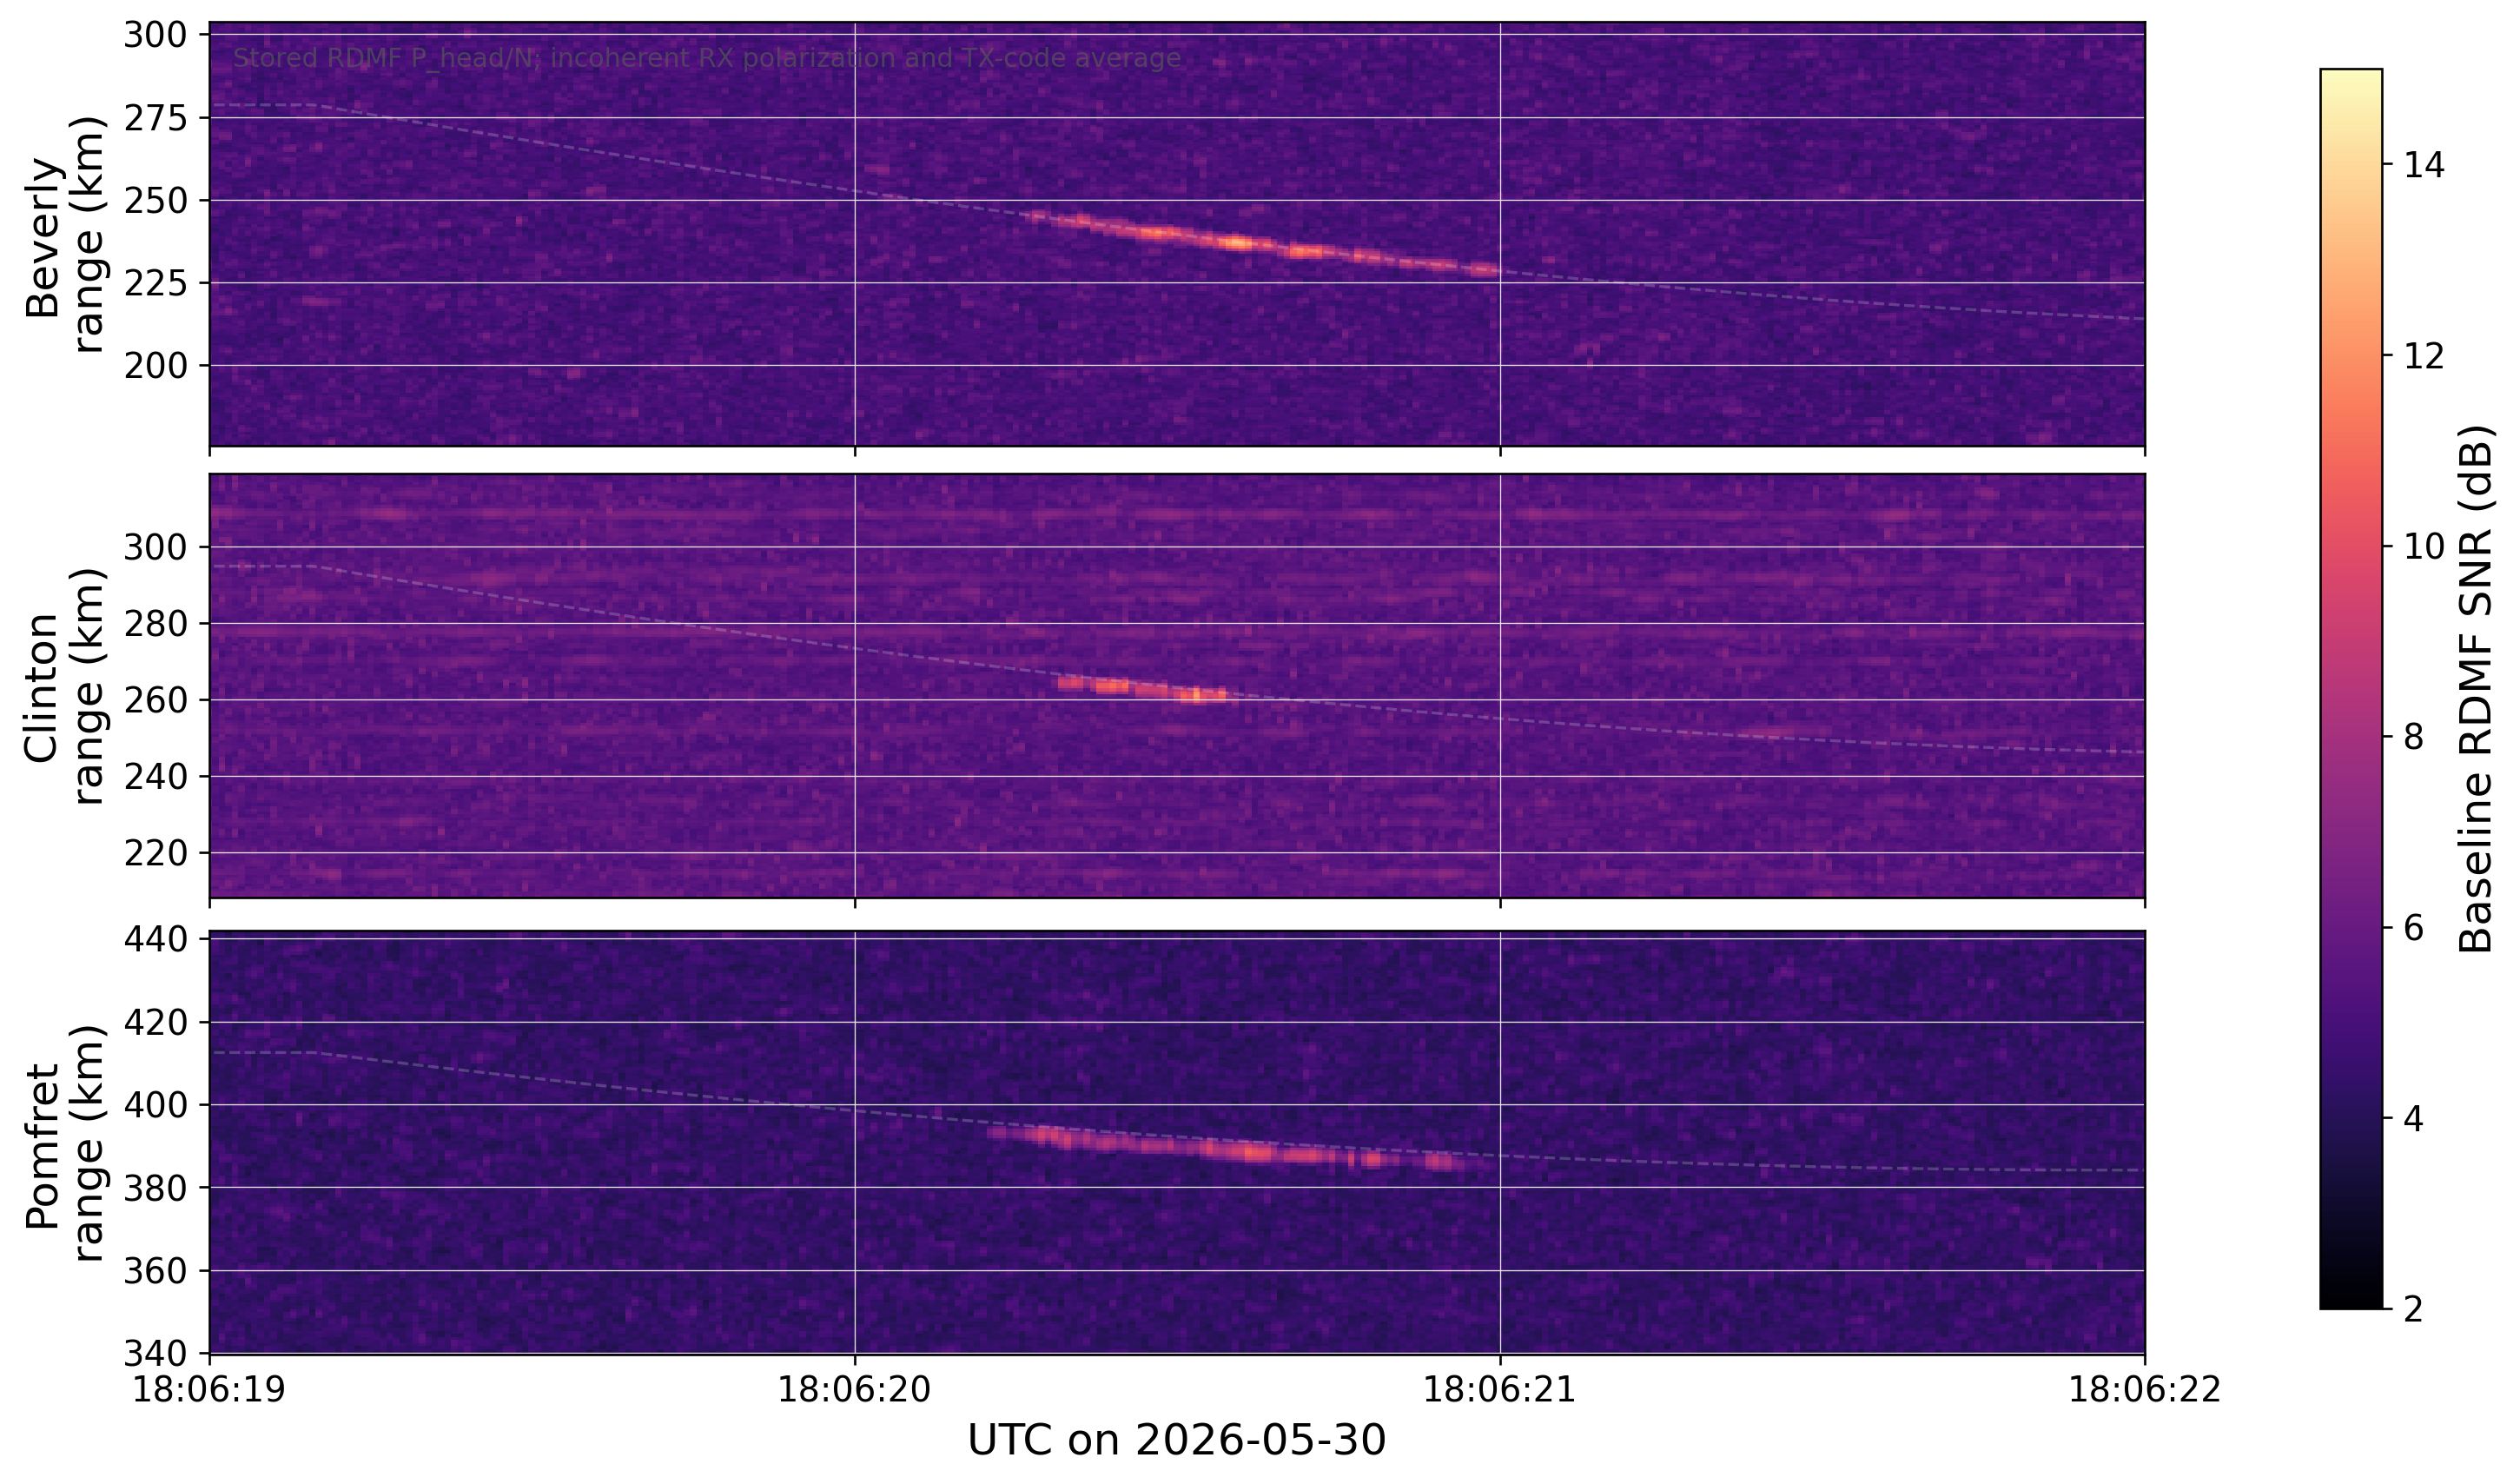
\includegraphics[width=\linewidth]{reports/figures/station_range_time_head_snr_rdmf_baseline.png}
  \caption{Baseline RDMF range--time SNR with incoherent averaging over
  transmitters and receive polarizations. \figsource{reports/generate_station_head_snr_rdmf_baseline.py}}
  \label{fig:v028-rdmf-baseline}
\end{figure}

\begin{figure}[H]
  \centering
  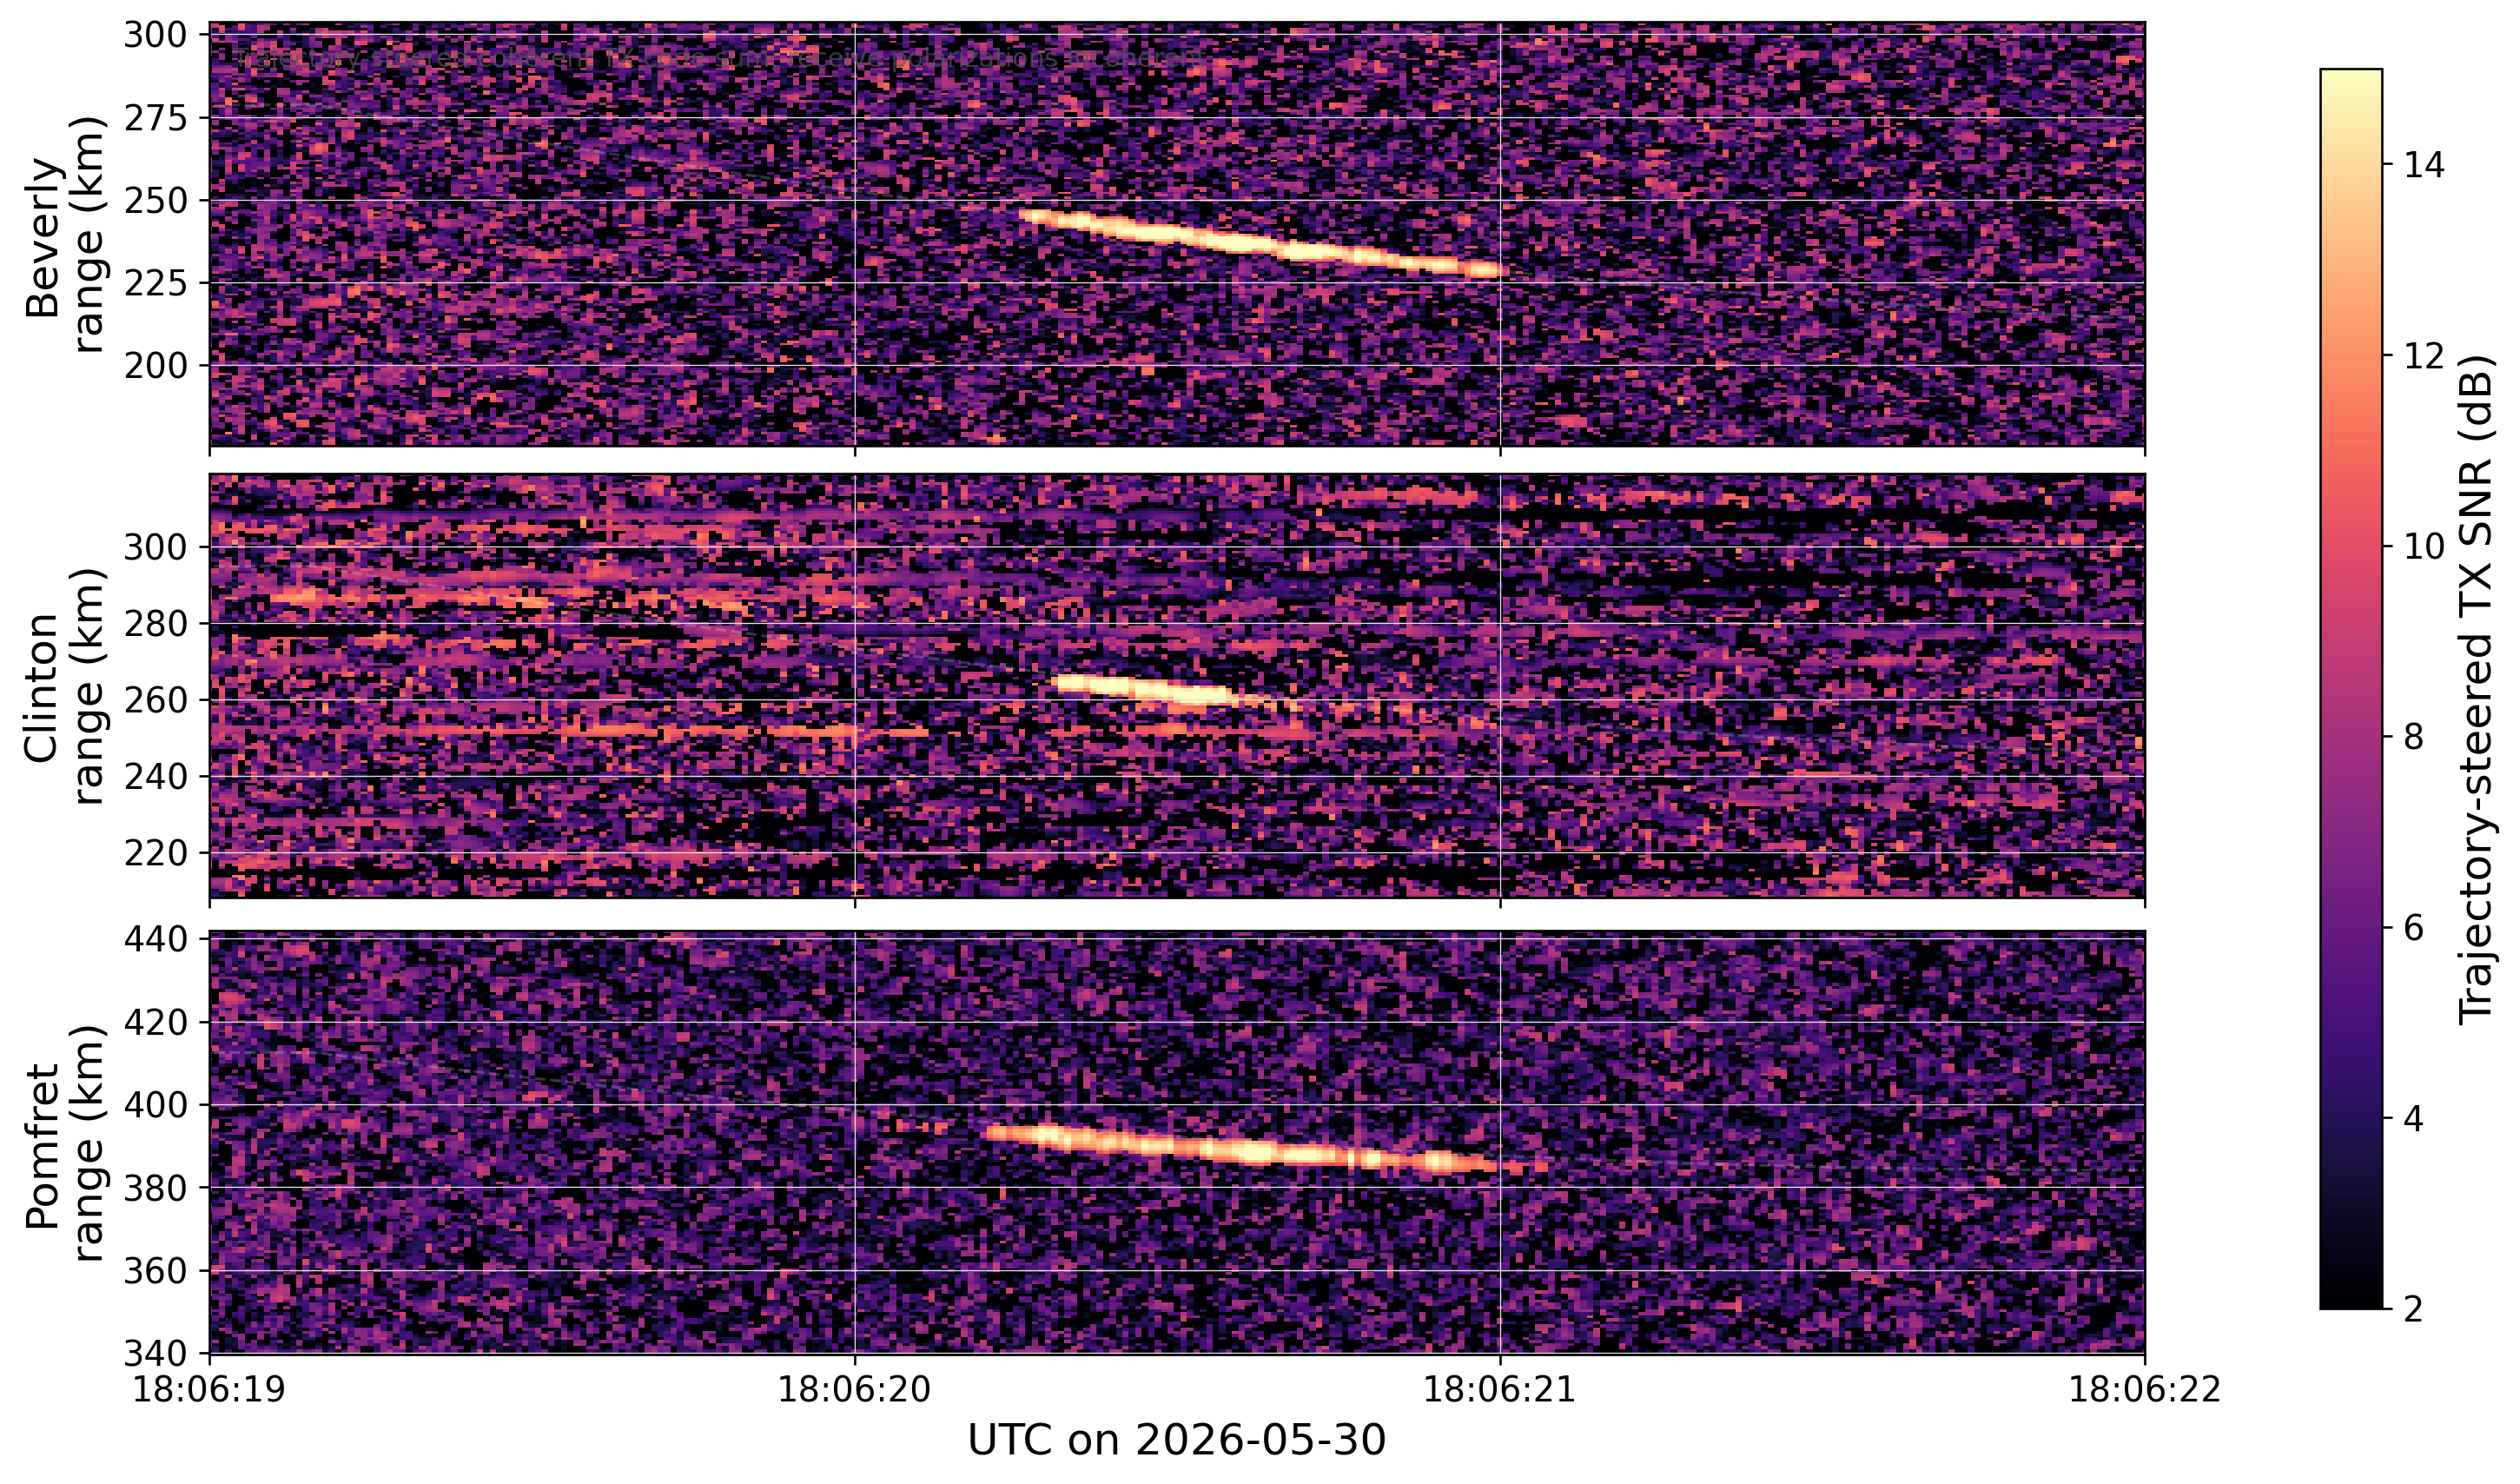
\includegraphics[width=\linewidth]{reports/figures/station_range_time_head_snr_rdmf_txsteer_incohpol.png}
  \caption{RDMF range--time SNR after trajectory-implied transmitter AoD
  steering, with receive polarizations still incoherently averaged.
  \figsource{reports/generate_station_head_snr_rdmf_baseline.py}}
  \label{fig:v028-rdmf-txsteer-incohpol}
\end{figure}

\begin{figure}[H]
  \centering
  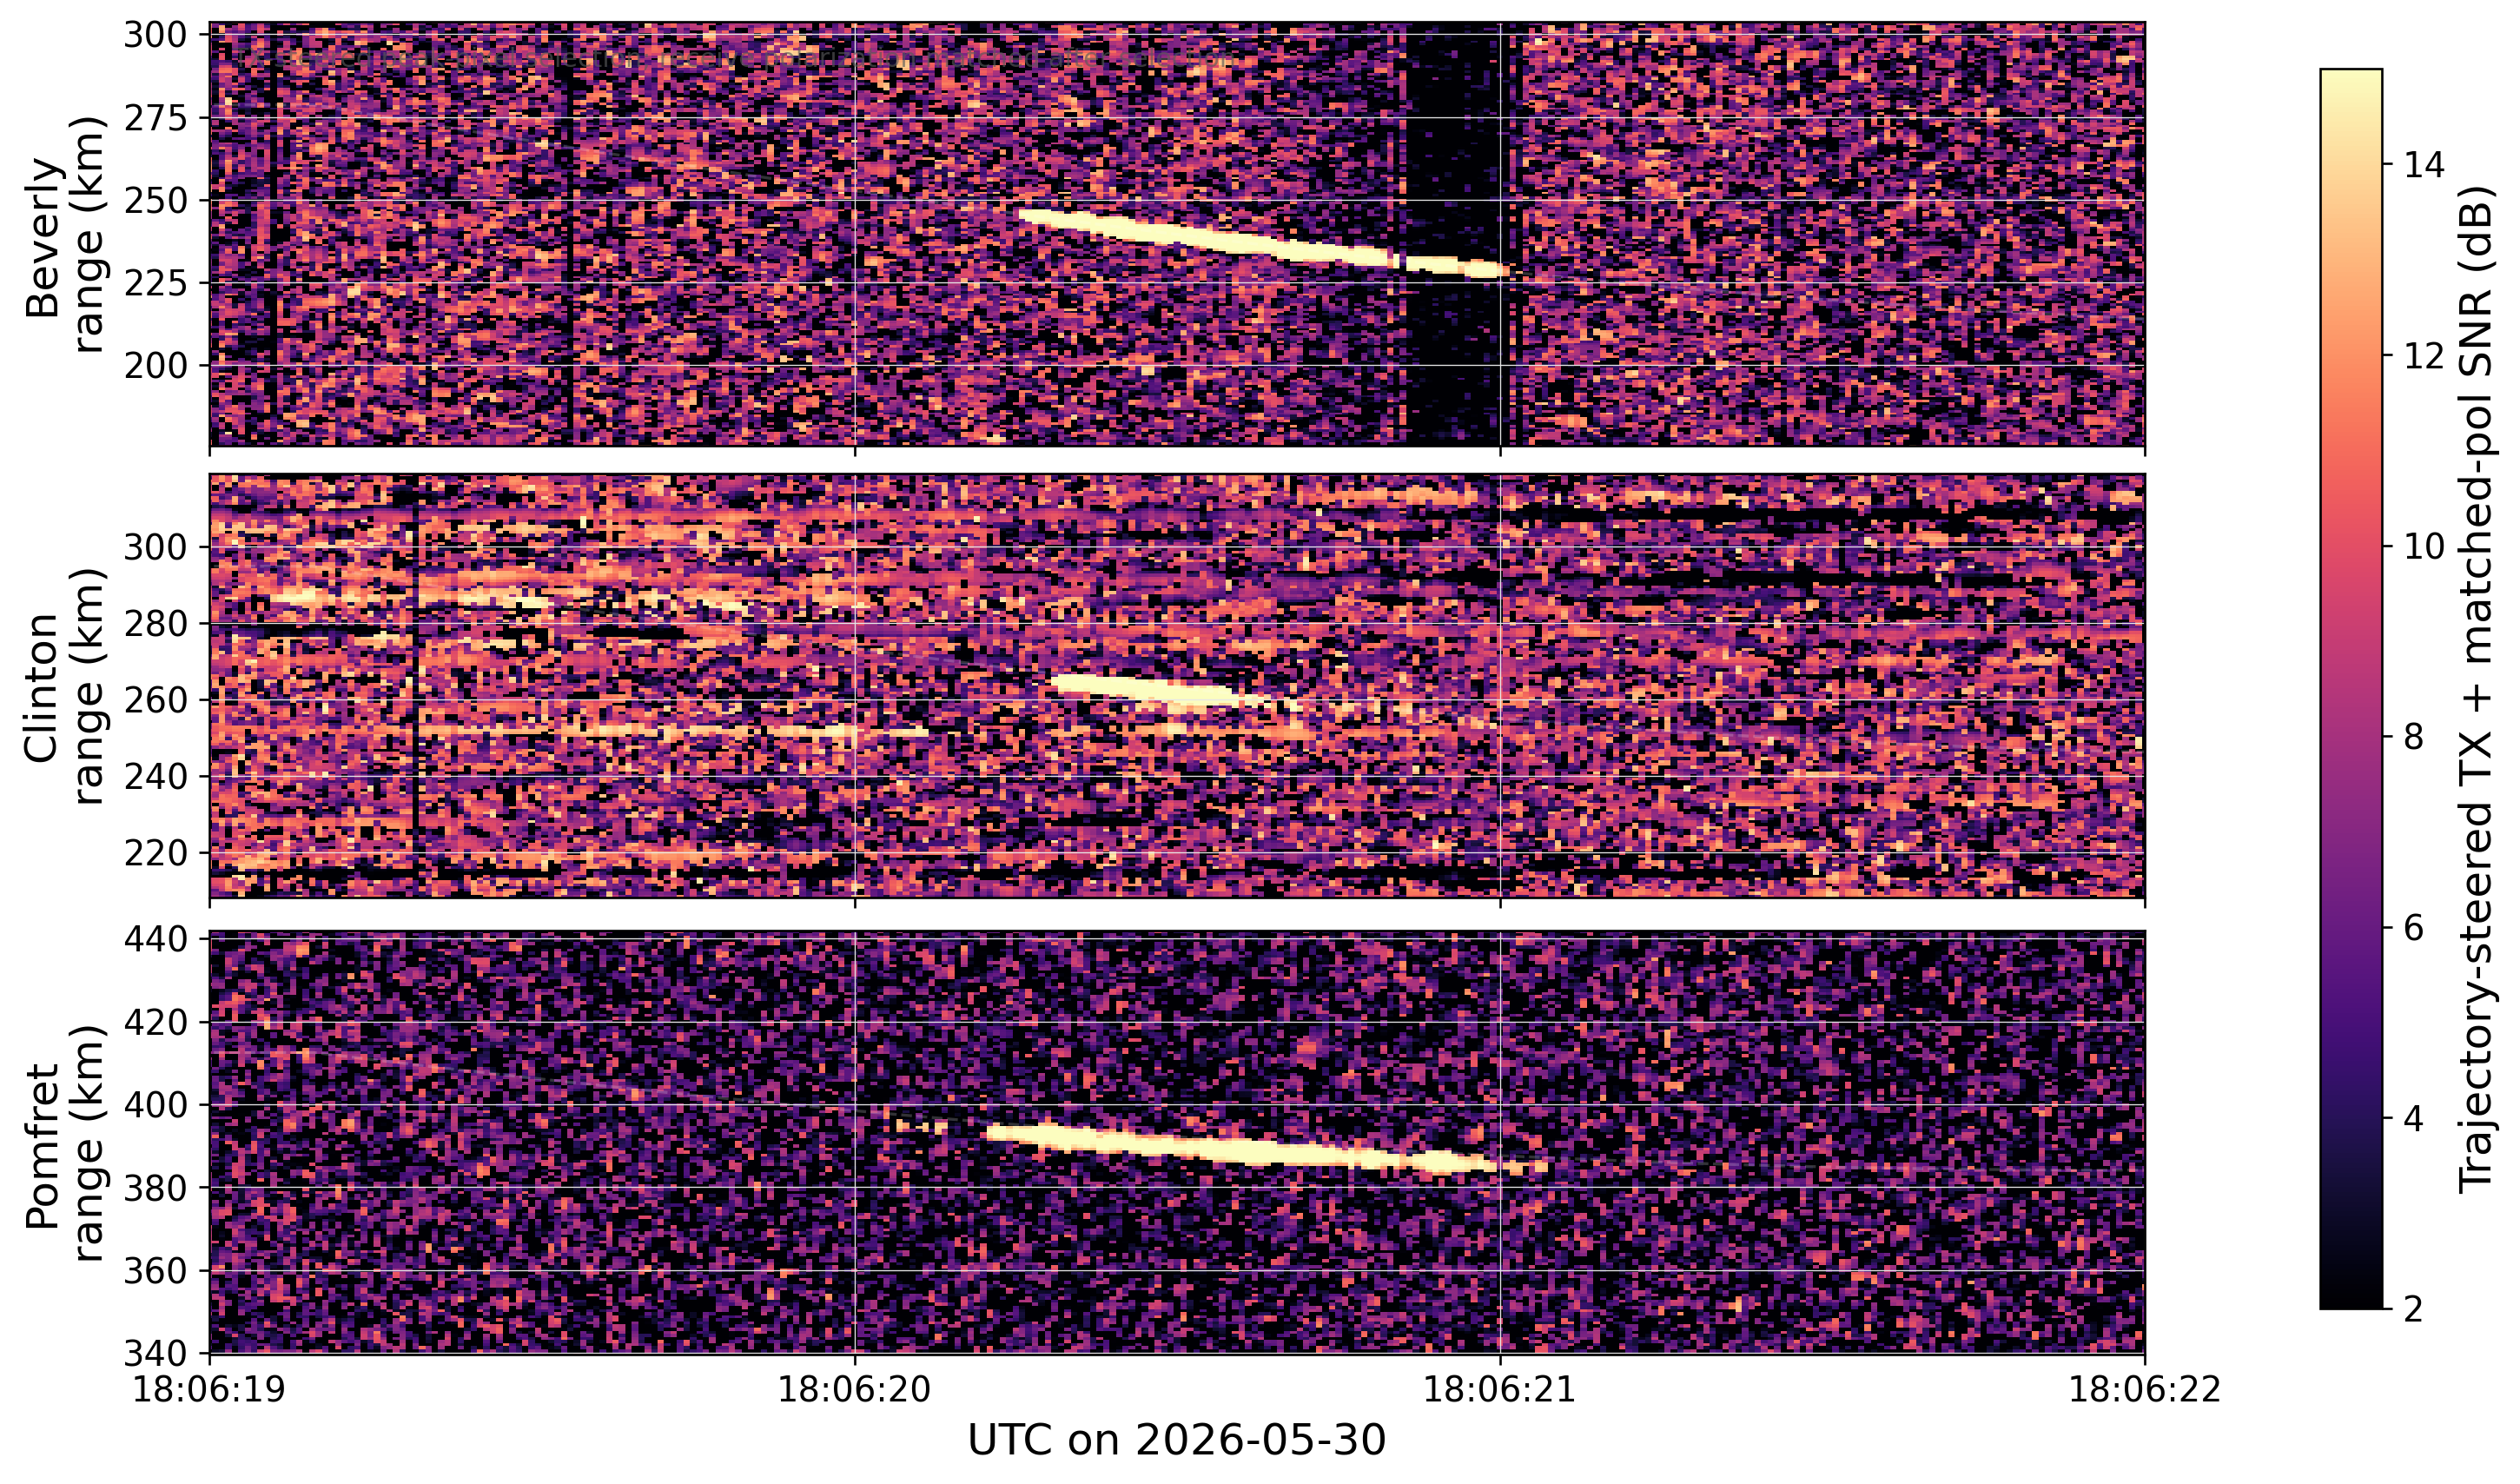
\includegraphics[width=\linewidth]{reports/figures/station_range_time_head_snr_rdmf_txsteer_polmatch.png}
  \caption{RDMF range--time SNR after trajectory-implied transmitter AoD
  steering and receive-polarization matching.  This is the combining order used
  for the v0.2.8 measurement-bank candidate products. \figsource{reports/generate_station_head_snr_rdmf_baseline.py}}
  \label{fig:v028-rdmf-txsteer-polmatch}
\end{figure}

\begin{figure}[H]
  \centering
  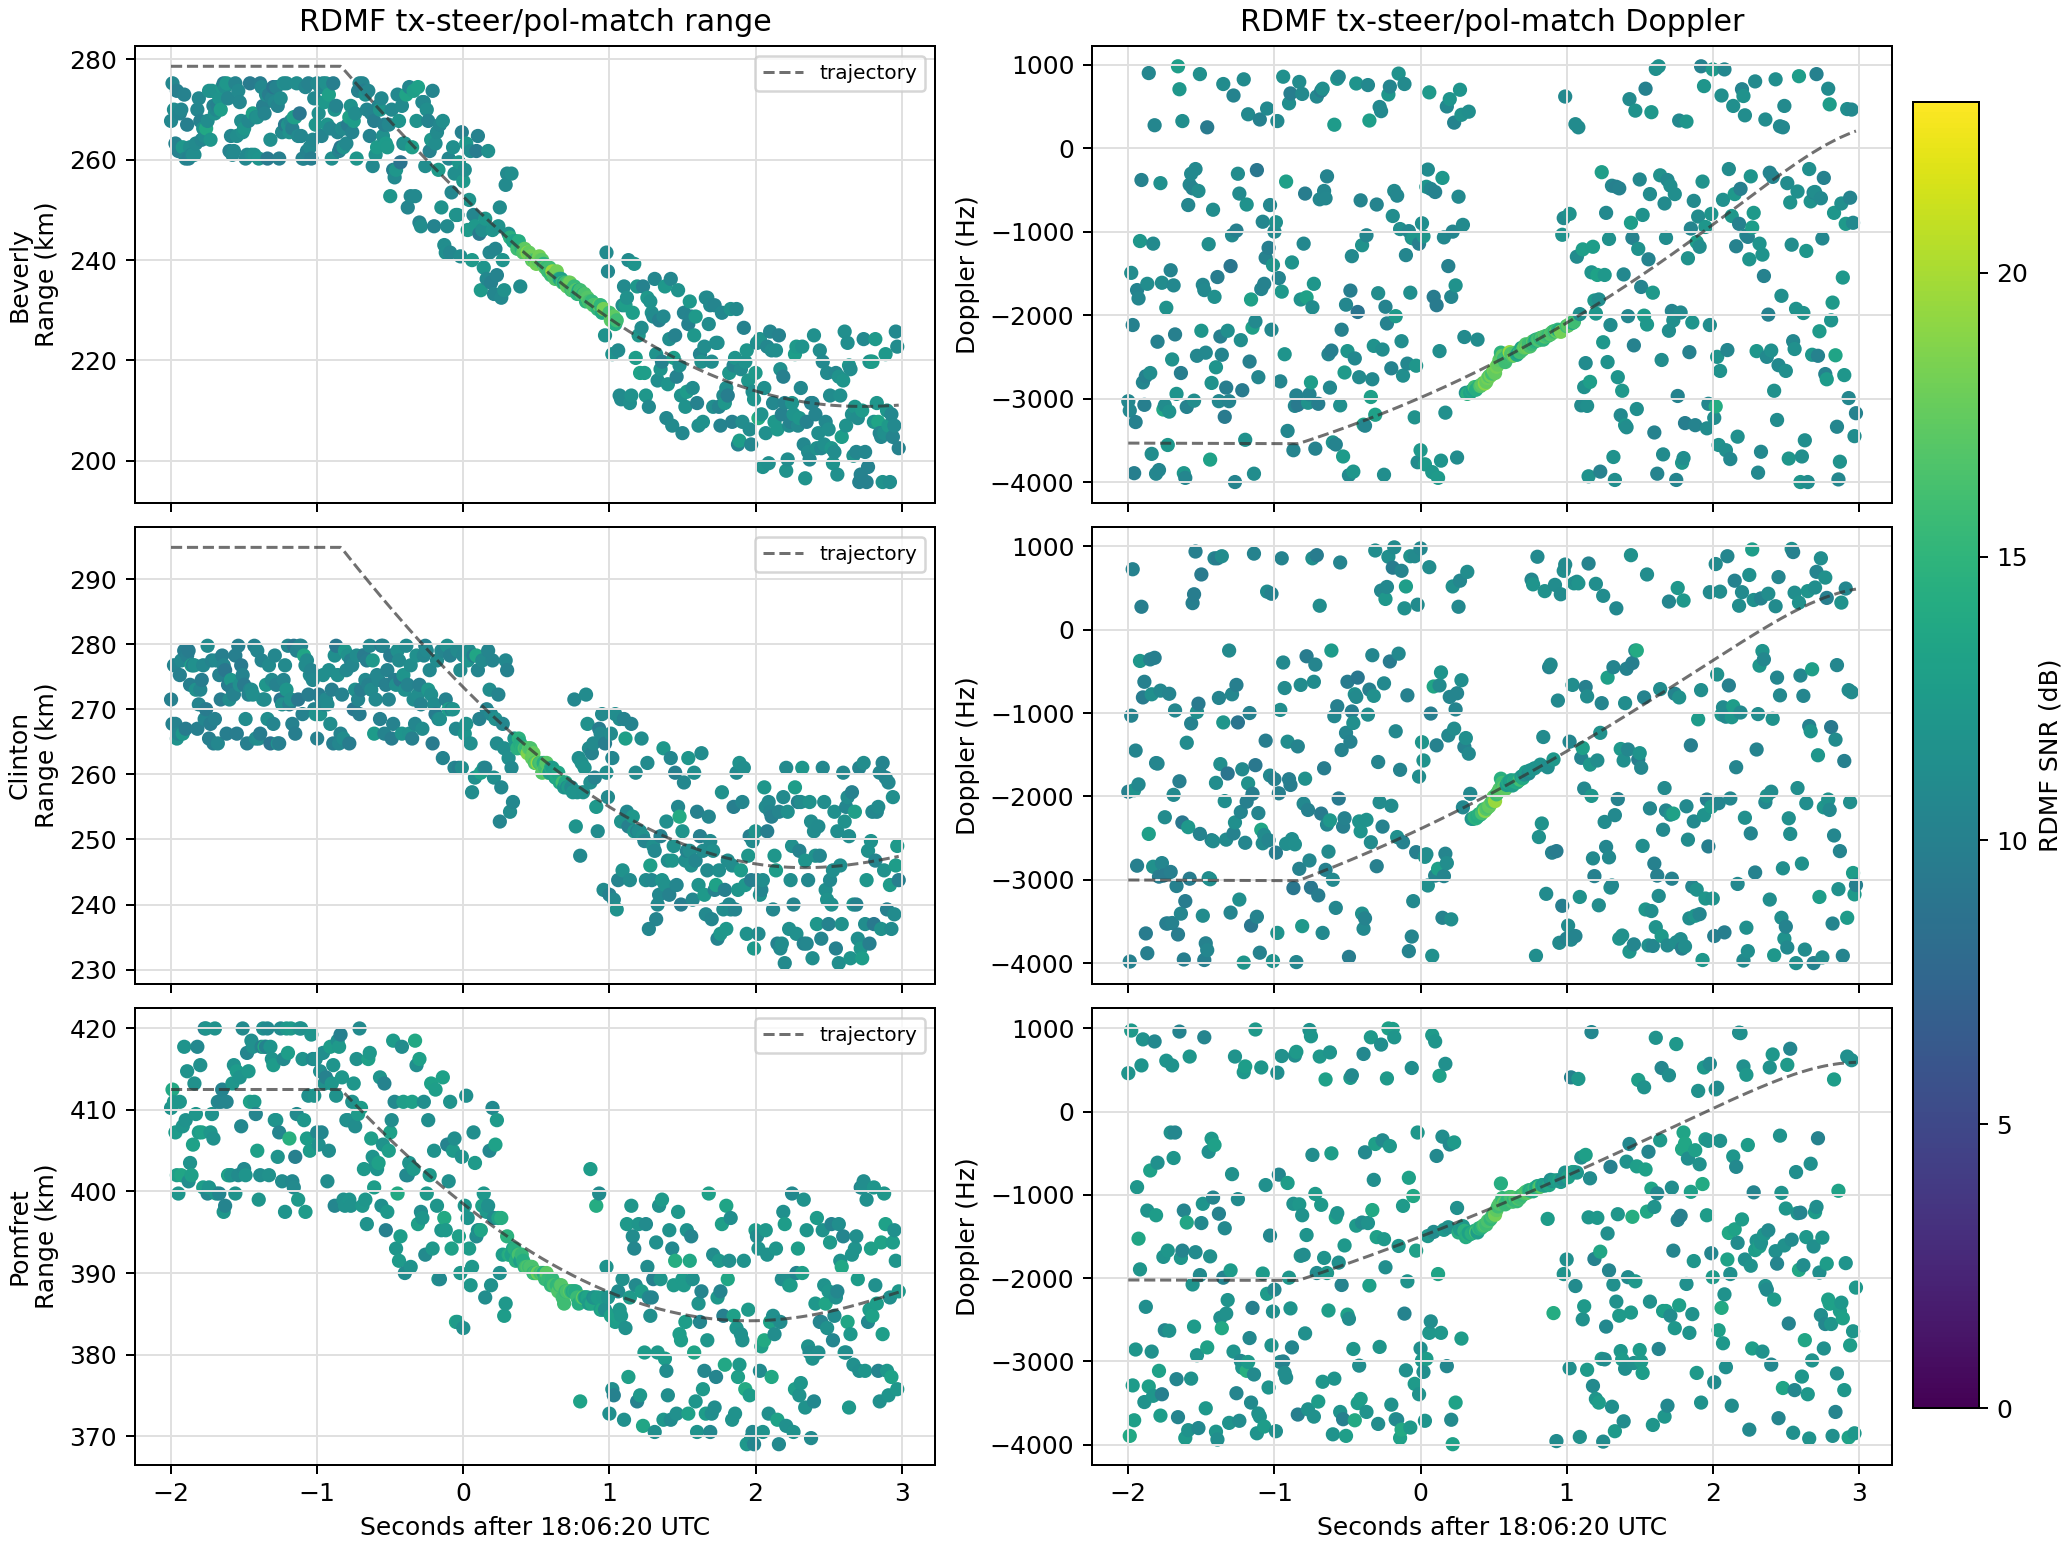
\includegraphics[width=\linewidth]{reports/figures/head_echo_rdmf_txsteer_pol_rinterp4_zp16_measurements_180618_180623.png}
  \caption{Selected v0.2.8 RDMF range and Doppler measurements from the
  trajectory-steered, polarization-matched measurement bank. \figsource{reports/generate_txsteer_pol_rdmf_measurements.py}}
  \label{fig:v028-rdmf-measurements}
\end{figure}

\section*{Measurement Selection and Ballistic Fit}

The GUI selection retained \CorrFitNHead{} head-echo observation epochs:
\CorrFitNHeadRange{} range measurements and \CorrFitNHeadDoppler{} Doppler
measurements.  The correlated ballistic fit also used \CorrFitNTrail{} trail
positions.  The resulting fit has \CorrFitNResiduals{} residuals and reduced
$\chi^2=\CorrFitReducedChiSq$.

\begin{figure}[H]
  \centering
  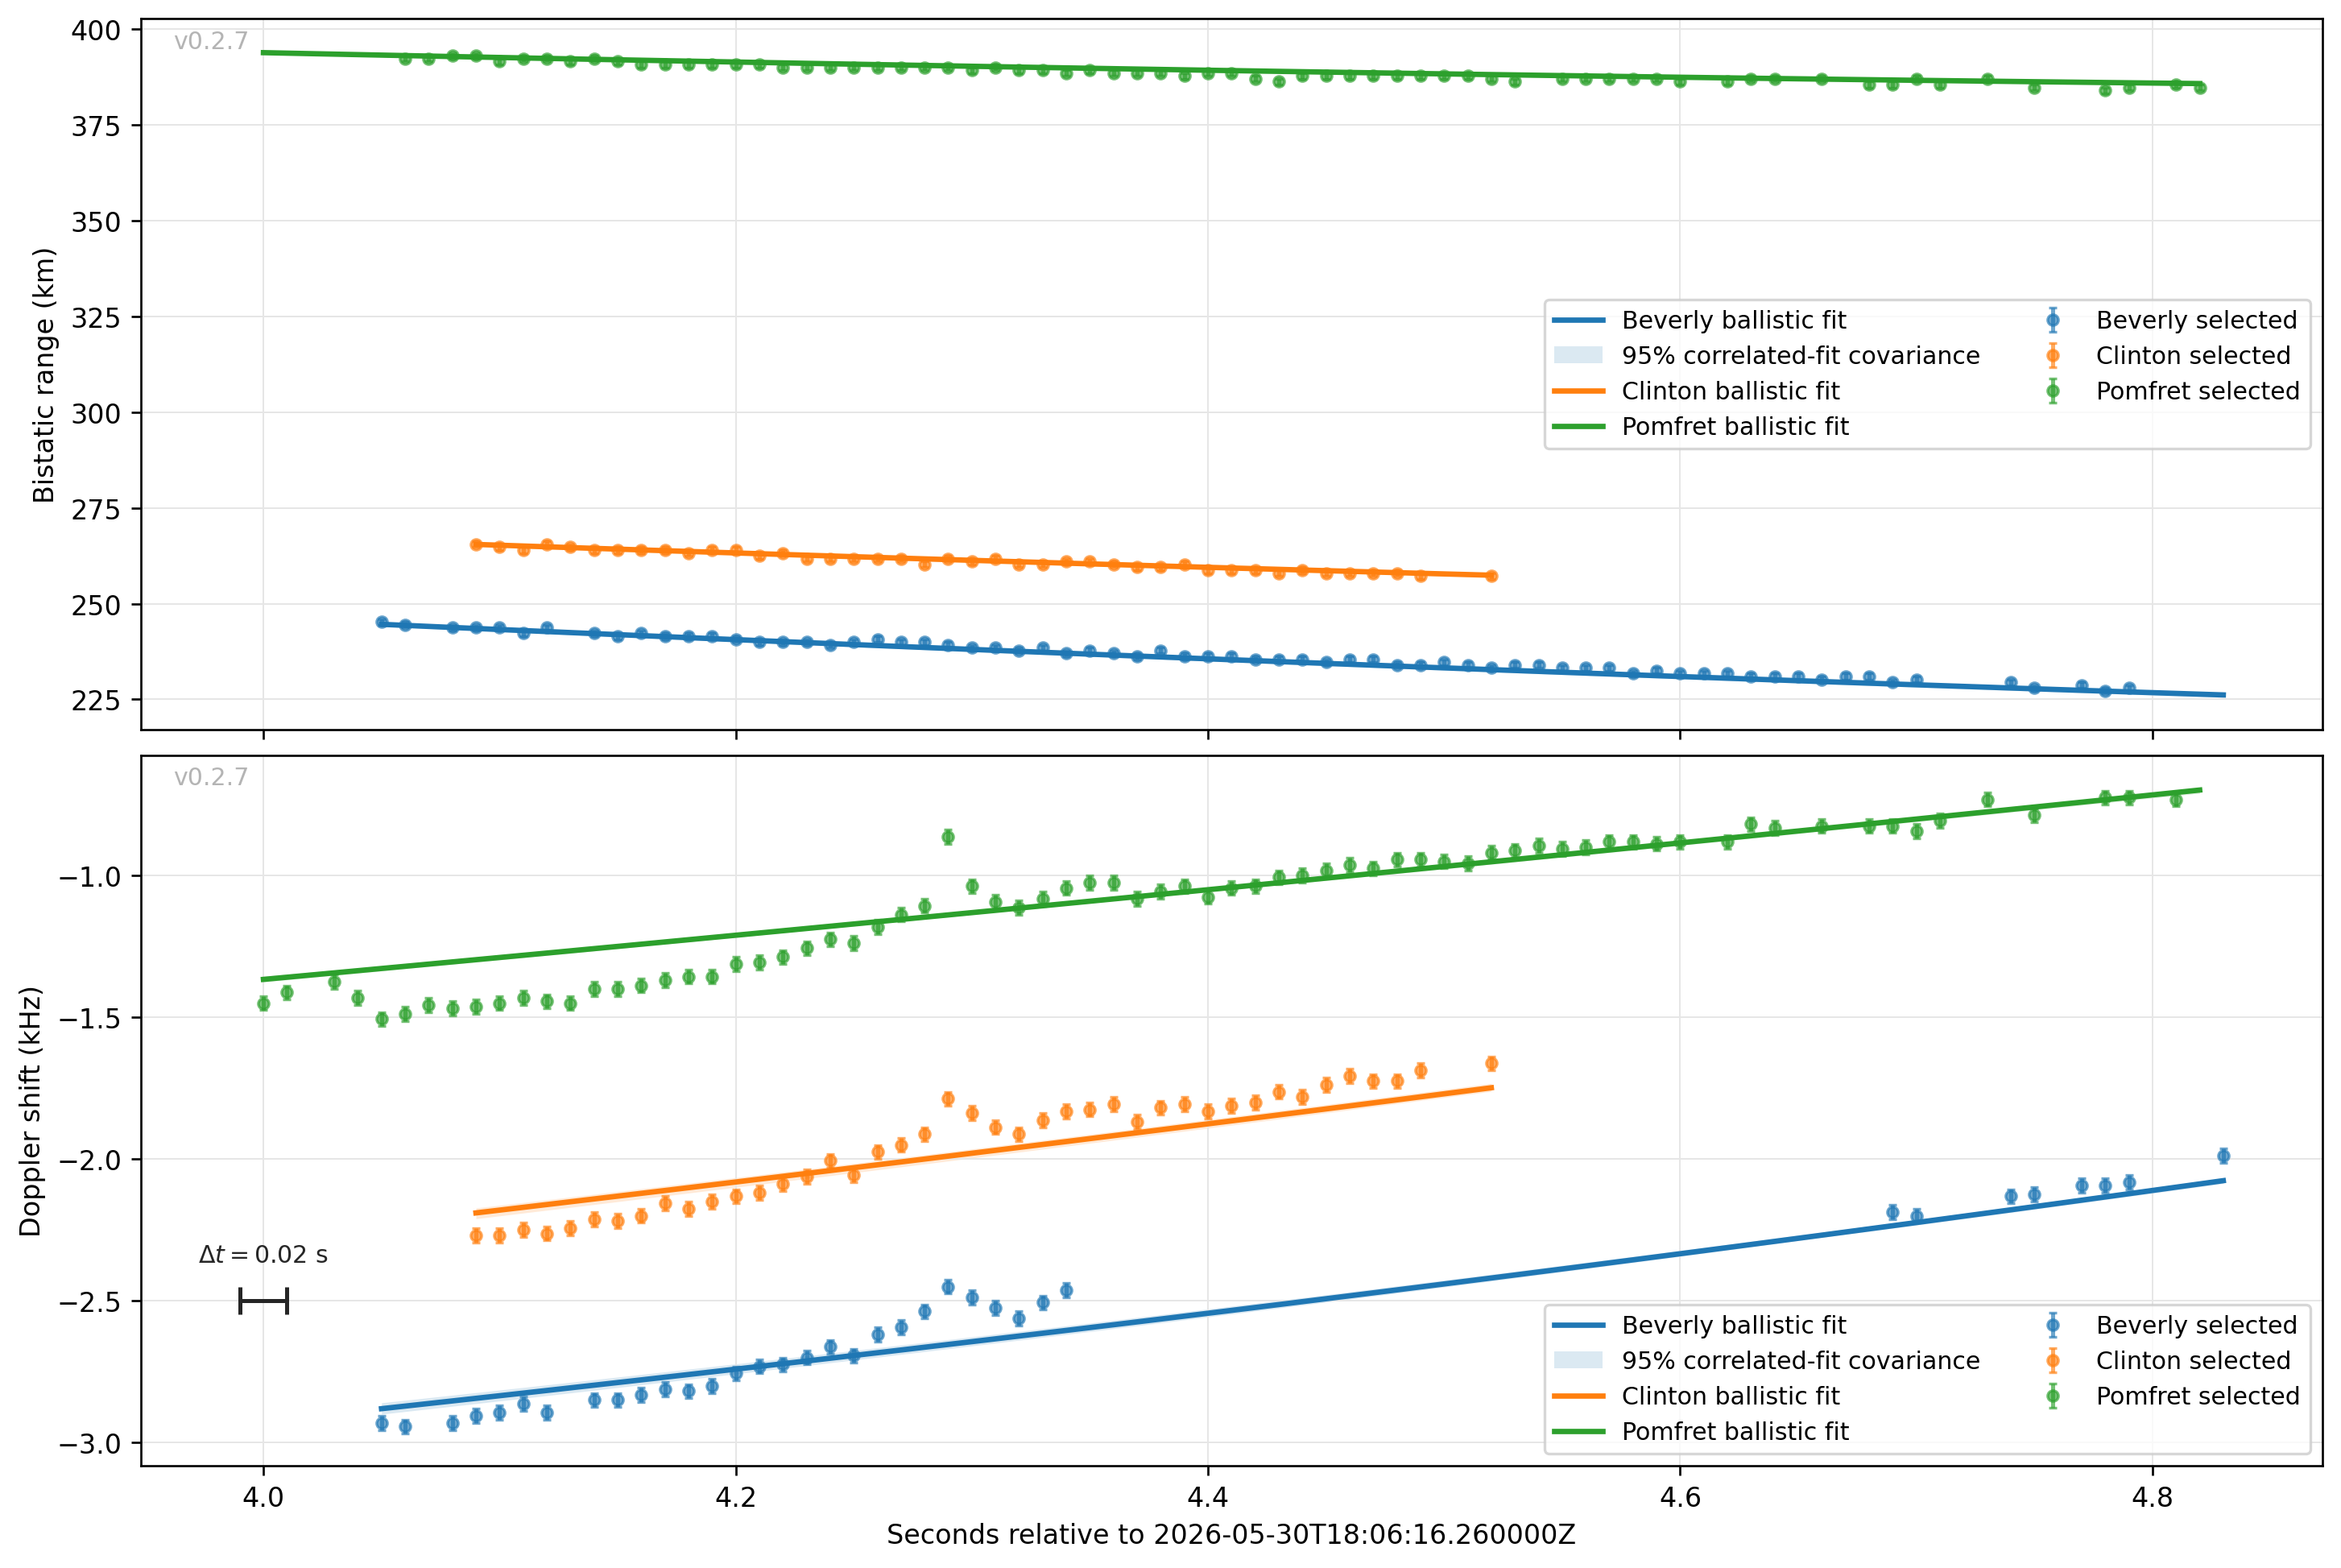
\includegraphics[width=\linewidth]{reports/figures/appendix_correlated_fit_v0p2p8_rinterp4_zp16/ballistic_head_trail_correlated_range_doppler_fit.png}
  \caption{Range and Doppler residual view for the v0.2.8 correlated
  ballistic fit. \figsource{fit_ballistic_head_trail_correlated_appendix.py}}
  \label{fig:v028-ballistic-range-doppler}
\end{figure}

\begin{figure}[H]
  \centering
  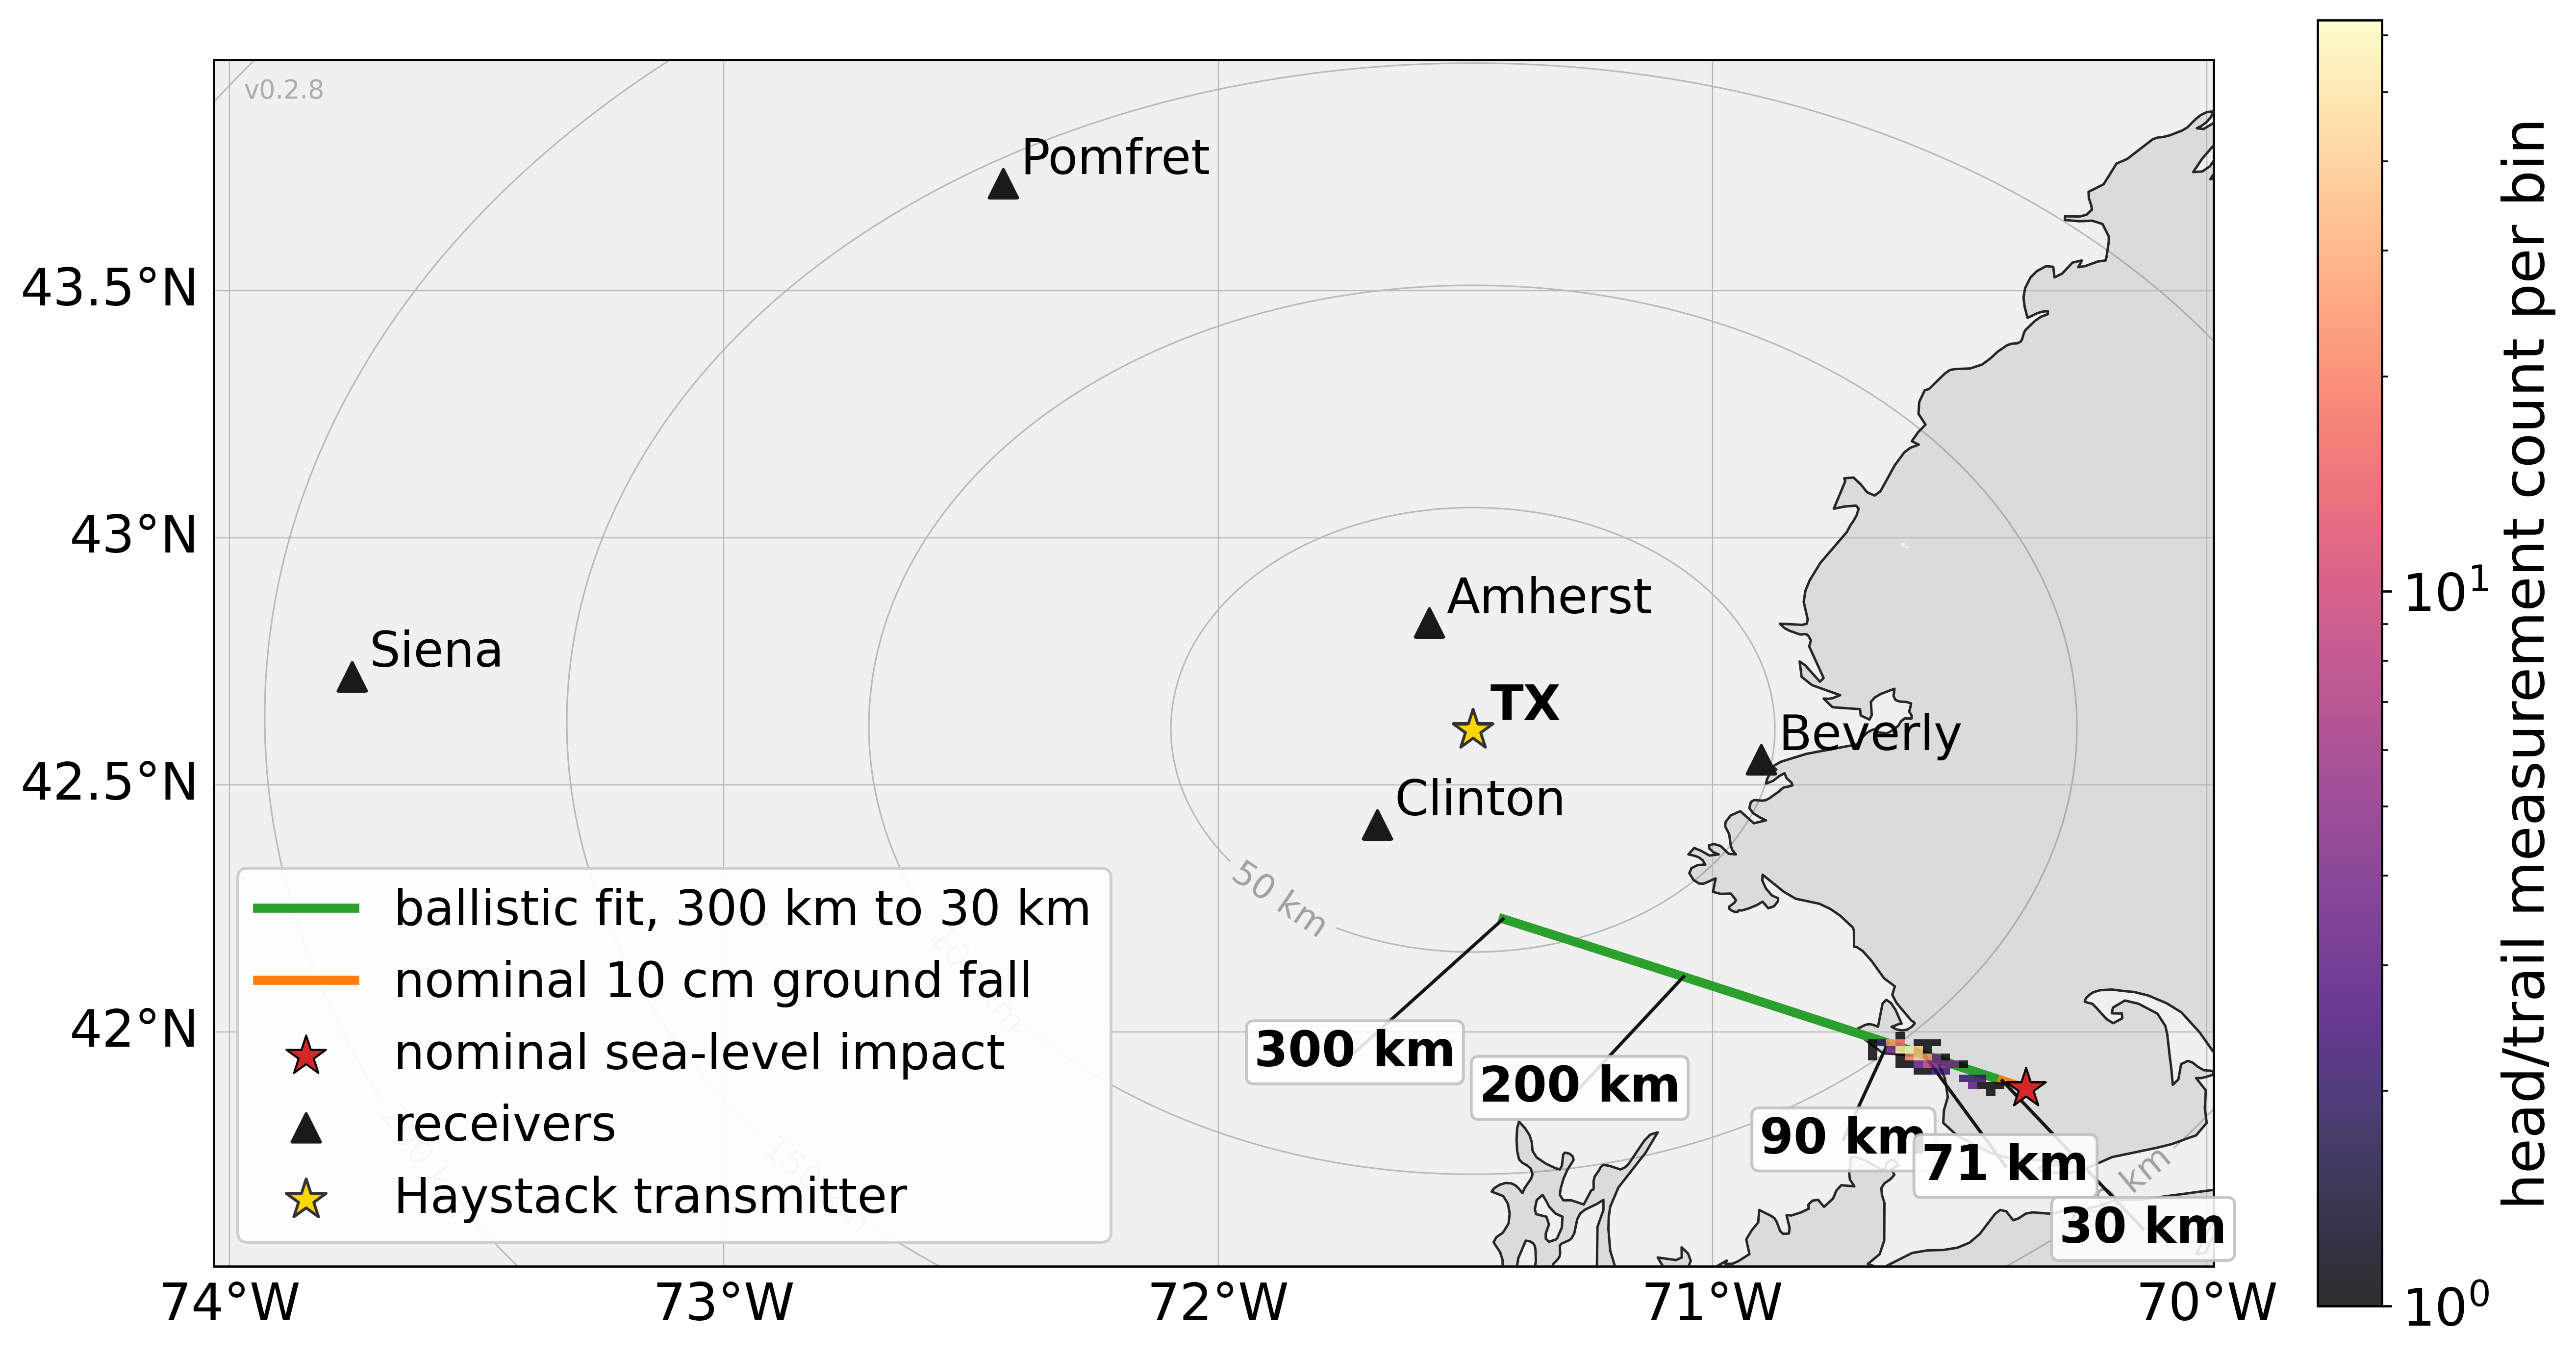
\includegraphics[width=\linewidth]{reports/figures/appendix_correlated_fit_v0p2p8_rinterp4_zp16/station_measurement_ballistic_correlated_overview.png}
  \caption{Station-wise v0.2.8 measurement overview used by the correlated
  ballistic fit. \figsource{fit_ballistic_head_trail_correlated_appendix.py}}
  \label{fig:v028-ballistic-station-overview}
\end{figure}

\noindent Ballistic fit product:
\path{products/ballistic_head_trail_correlated_fit_v0p2p8_rinterp4_zp16/ballistic_head_trail_correlated_fit.json}

\noindent Initial state used for orbit sampling:
\path{products/ballistic_head_trail_correlated_fit_v0p2p8_rinterp4_zp16/ballistic_initial_state_correlated.json}

\section*{Orbit Determination}

The v0.2.8 correlated ballistic initial state was propagated through the orbit
determination sampler with 2000 Monte Carlo samples in the \texttt{rebound}
conda environment.  The resulting orbit sample is tied to trajectory fit
version \OrbitTrajectoryFitVersion{} and epoch \OrbitEpochUTC{}.

\begin{figure}[H]
  \centering
  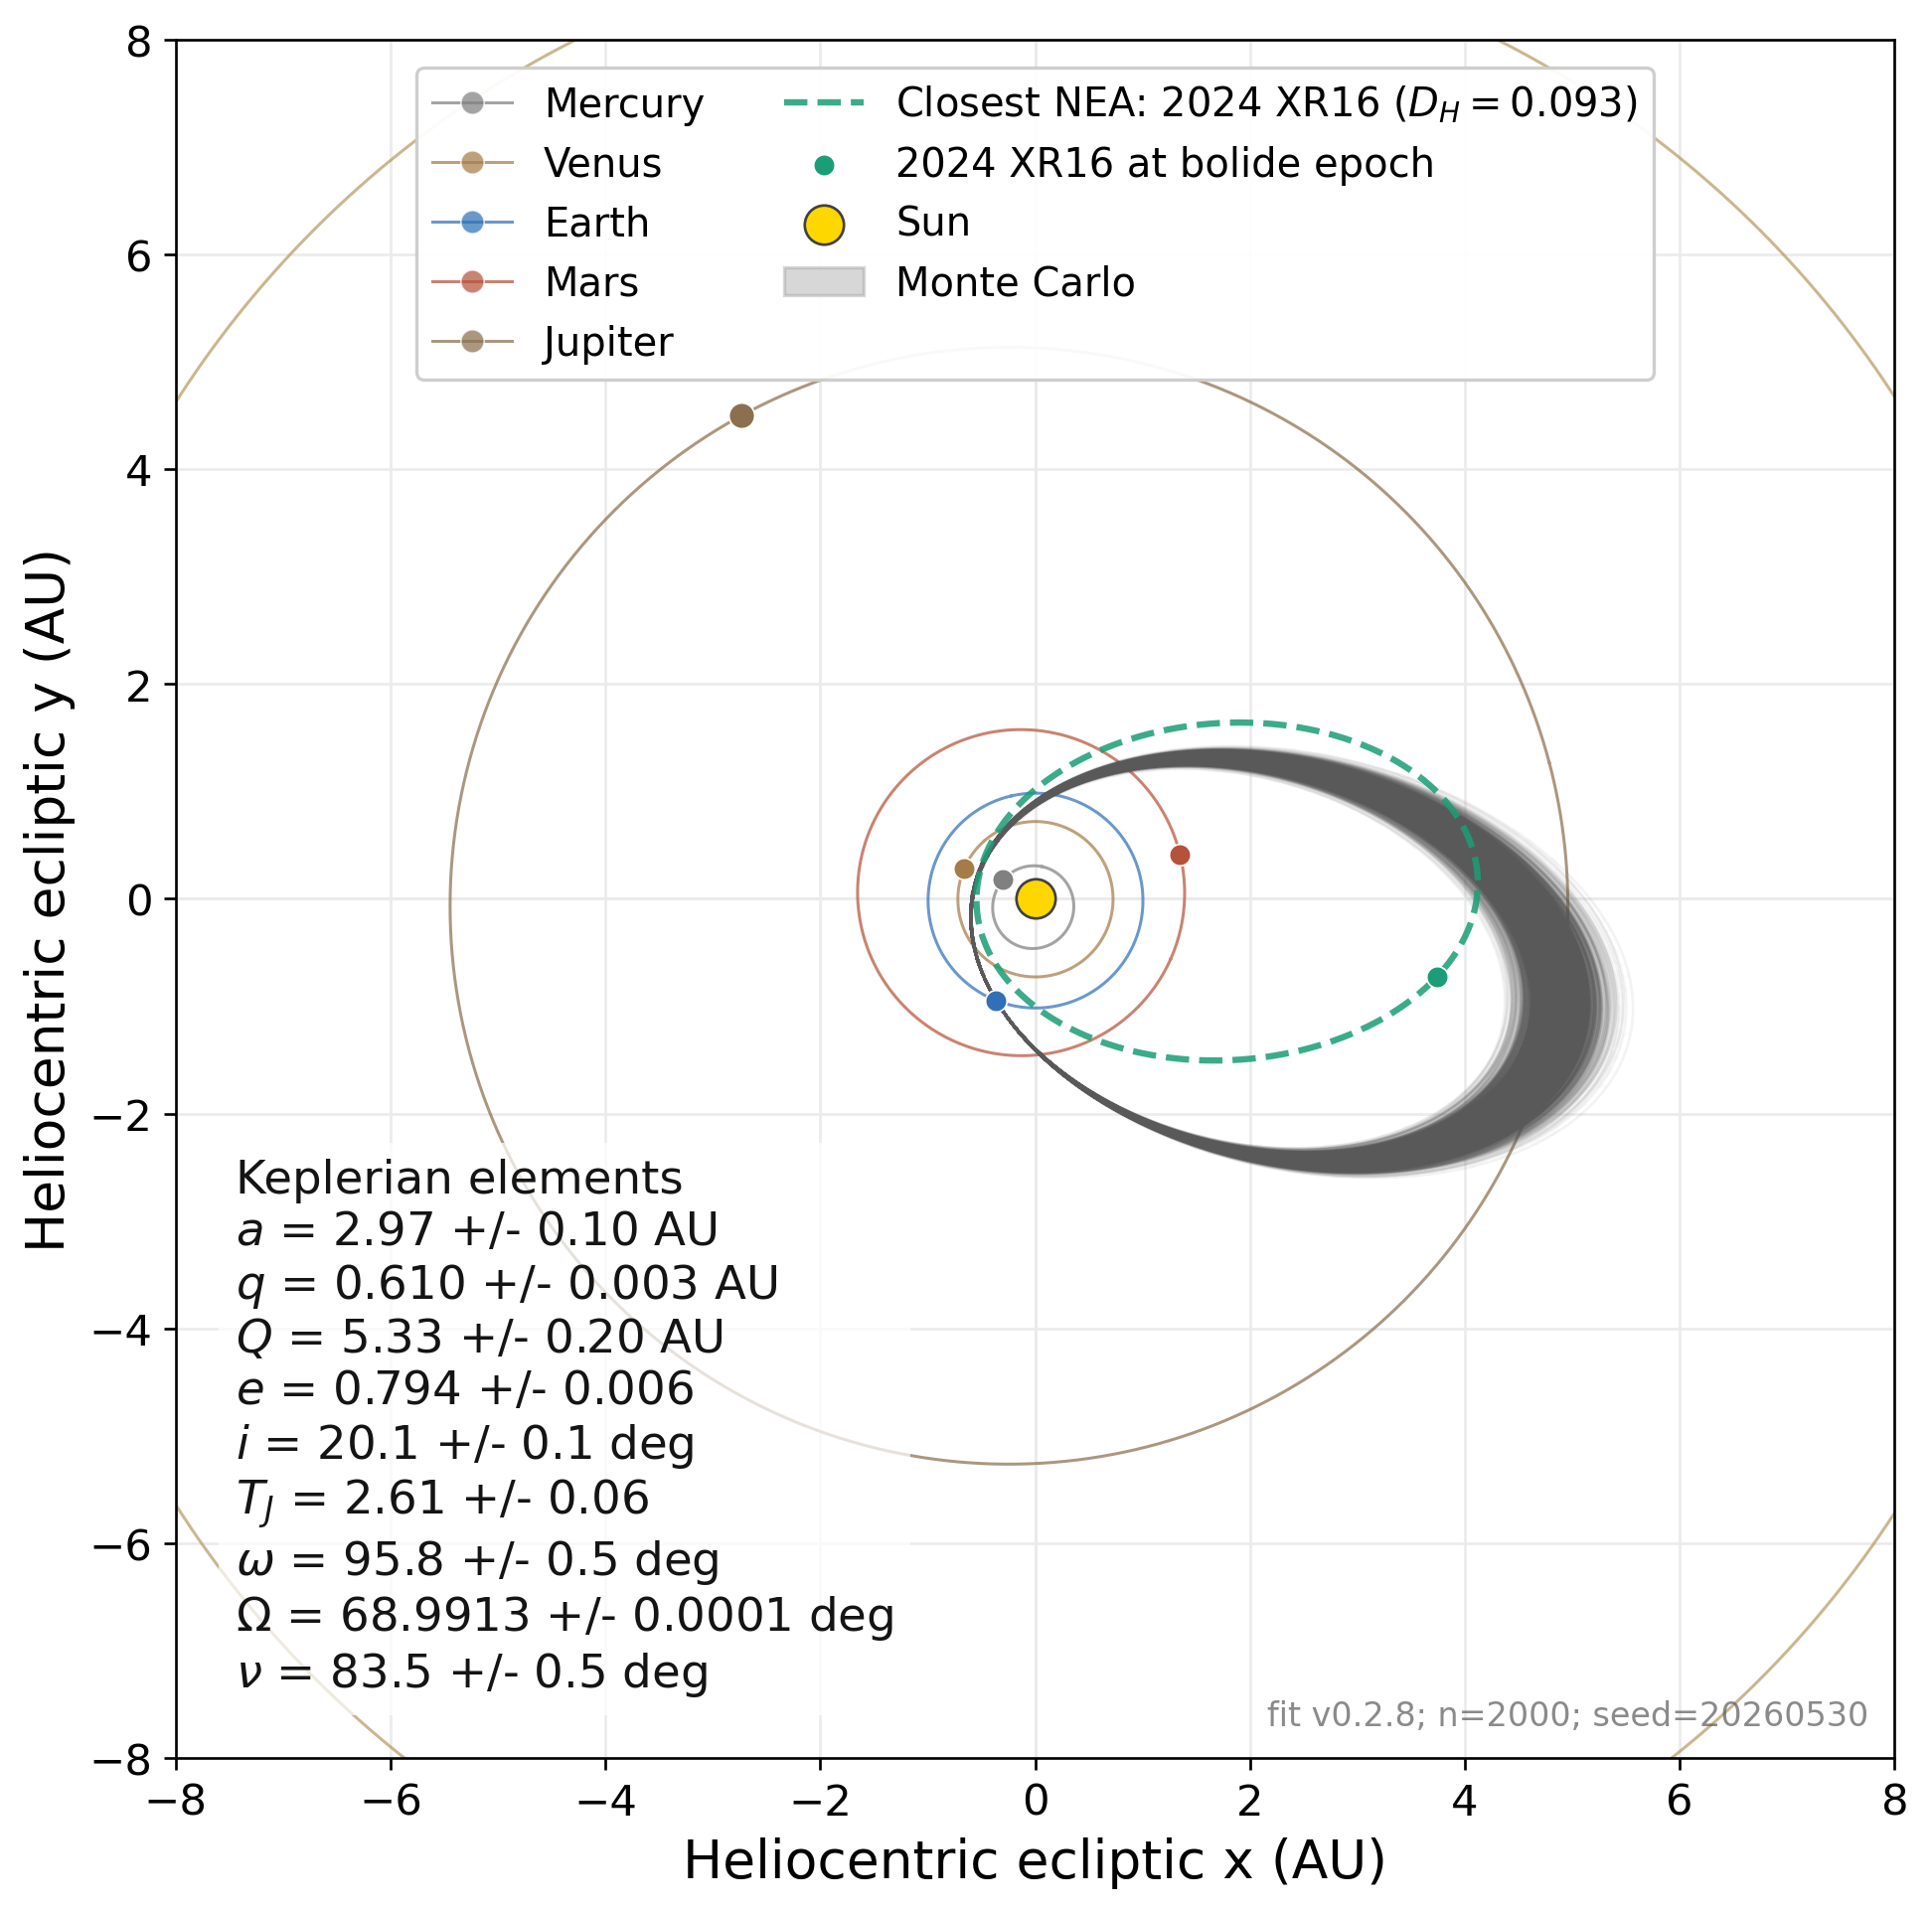
\includegraphics[width=0.88\linewidth]{reports/figures/orbit_xy_bolide_v0p2p8_rinterp4_zp16.png}
  \caption{Heliocentric ecliptic $x$--$y$ orbit plot for the v0.2.8
  trajectory-steered and polarization-matched RDMF selection. \figsource{plot_orbit_xy.py}}
  \label{fig:v028-orbit-xy}
\end{figure}

\begin{center}
% trajectory_fit_version: 0.2.8
% trajectory_fit_version_description: Selected head-echo correlated ballistic fit using AoD-steered TX combining, receive-polarization matching, range interpolation by 4, 16x FFT over the interpolated code length, sparse-fit residual voltage, and manual range/Doppler selections from the rinterp4/zp16 RDMF candidate GUI.
\begin{tabular}{llrl}
\toprule
Quantity & Symbol & Unit & Estimate {\footnotesize (v0.2.8)} \\
\midrule
Semimajor axis & $a$ & AU & 2.97 $\pm$ 0.10 \\
Perihelion distance & $q$ & AU & 0.6103 $\pm$ 0.0027 \\
Aphelion distance & $Q$ & AU & 5.33 $\pm$ 0.20 \\
Eccentricity & $e$ &  & 0.794 $\pm$ 0.006 \\
Inclination & $i$ & deg & 20.14 $\pm$ 0.14 \\
Argument of perihelion & $\omega$ & deg & 95.8 $\pm$ 0.5 \\
Longitude of ascending node & $\Omega$ & deg & 68.99132 $\pm$ 0.00011 \\
True anomaly at epoch & $\nu$ & deg & 83.5 $\pm$ 0.5 \\
Geocentric speed & $v_g$ & km s$^{-1}$ & 24.94 $\pm$ 0.14 \\
Tisserand parameter with respect to Jupiter & $T_J$ &  & 2.61 $\pm$ 0.06 \\
Corrected radiant right ascension & RA & deg & 60.08 $\pm$ 0.26 \\
Corrected radiant declination & Dec & deg & 46.61 $\pm$ 0.17 \\
Time at 100 km & $t_{100}$ & UTC & 2026-05-30 18:06:19.842 UTC \\
Geodetic latitude at 100 km & $\phi_{100}$ & deg & 41.99 \\
Geodetic longitude at 100 km & $\lambda_{100}$ & deg & -70.68 \\
Entry azimuth at 100 km & Az$_{100}$ & deg & 113.7 \\
Entry elevation at 100 km & El$_{100}$ & deg & -70.7 \\
Velocity at 100 km & $v_{100}$ & km s$^{-1}$ & 26.88 \\
\bottomrule
\end{tabular}

\end{center}

\begin{center}
% Generated by reports/generate_orbit_classification_table.py; do not edit by hand.
% trajectory_fit_version: 0.2.8
% orbit_sample_source: products/orbit_determination_v0p2p8_rinterp4_zp16/best_fit_orbit.h5
% orbit_sample_selection: all 2000 finite samples
% trajectory_json: products/ballistic_head_trail_correlated_fit_v0p2p8_rinterp4_zp16/ballistic_initial_state_correlated.json
\begin{tabular}{llrr}
\toprule
\multicolumn{4}{l}{Fit version v0.2.8; 2000 finite orbit samples} \\
\midrule
Criterion & Quantity & Cometary & Asteroidal \\
\midrule
$T_J-i$ & Tisserand parameter with respect to Jupiter & 100.0\% & 0.0\% \\
$K-i$ & Semimajor-axis--eccentricity criterion & 100.0\% & 0.0\% \\
$Q-i$ & Aphelion-distance criterion & 100.0\% & 0.0\% \\
$P-i$ & Orbital-period criterion & 100.0\% & 0.0\% \\
$\varepsilon-i$ & Specific-orbital-energy criterion & 96.0\% & 3.9\% \\
\bottomrule
\end{tabular}

\end{center}

\noindent Orbit sample:
\path{products/orbit_determination_v0p2p8_rinterp4_zp16/best_fit_orbit.h5}

\noindent Orbit eccentricity diagnostic:
\path{products/orbit_determination_v0p2p8_rinterp4_zp16/best_fit_orbit_eccentricity_HeliocentricMeanEcliptic.png}

\noindent Orbit source table:
\path{reports/orbit_source_table_v0p2p8_rinterp4_zp16.tex}

\section*{Source Programs}

\begin{itemize}
  \item \texttt{\detokenize{range_doppler_mf_bolide.py}}
  \item \texttt{\detokenize{reports/run_txsteer_pol_rdmf_measurement_bank.py}}
  \item \texttt{\detokenize{reports/generate_txsteer_pol_rdmf_measurements.py}}
  \item \texttt{\detokenize{reports/generate_station_head_snr_rdmf_baseline.py}}
  \item \texttt{\detokenize{reports/select_head_echo_measurements.py}}
  \item \texttt{\detokenize{fit_ballistic_head_trail_correlated_appendix.py}}
  \item \texttt{\detokenize{orbit_det_sample.py}}
  \item \texttt{\detokenize{reports/generate_orbit_source_table.py}}
  \item \texttt{\detokenize{reports/generate_orbit_classification_table.py}}
  \item \texttt{\detokenize{plot_orbit_xy.py}}
\end{itemize}

\end{document}
